\section{Trực quan hóa mô hình hồi quy động học}
\label{sec:nonlinear_regression_plot}

Trong phân tích dữ liệu cảm biến tự động, sau khi thuật toán \texttt{curve\_fit} hoàn tất việc ước lượng các tham số vật lý và tính ma trận hiệp phương sai, việc vẽ đồ thị hồi quy là bước kiểm tra trực quan quan trọng. Thao tác này thể hiện mức độ phù hợp giữa mô hình toán học dự đoán và tập dữ liệu thực nghiệm (bao gồm các điểm dữ liệu và thanh sai số tương ứng). Khi áp dụng vào bài toán minh họa, ta tiến hành vẽ đồ thị song song cho cả mô hình phi tuyến đối với độ dịch chuyển và mô hình tuyến tính đối với vận tốc.

\begin{physcore}{Độ phân giải trục hoành trong nội suy đồ thị}{interpolation_resolution}
Trong môi trường vẽ đồ thị khoa học của Python, một hàm toán học liên tục không được hiển thị trực tiếp thông qua một công thức giải tích. Thay vào đó, hàm này được xấp xỉ bằng một tập hợp các điểm rời rạc nối tiếp nhau. Nếu mảng thời gian lấy mẫu (\texttt{time\_data}) được sử dụng trực tiếp làm trục hoành để vẽ đường mô hình hồi quy, đặc biệt đối với các hệ thống có tần số lấy mẫu thưa thớt, đường cong biểu diễn dễ xuất hiện hiện tượng đứt gãy dạng đa giác (polygonal artifacts). Để duy trì tính liên tục trơn tru của hàm phi tuyến về mặt thị giác, việc thiết lập một lưới điểm nội suy mới với độ phân giải cao hơn (thông qua các hàm tạo mảng như \texttt{np.linspace}) là một bước cần thiết.
\end{physcore}

Đoạn mã dưới đây minh họa phương pháp kết hợp đồng thời hai mô hình hồi quy động học trên một cấu trúc đồ thị phân nhánh. Các thông số thống kê cốt lõi, bao gồm phương trình mô hình tối ưu, ước lượng gia tốc trọng trường $g$ kèm theo độ lệch chuẩn và hệ số xác định $R^2$, được tự động chèn vào các hộp thông tin (parameter boxes) thông qua chuỗi định dạng (f-strings) kết hợp cú pháp LaTeX.

\begin{pycode}{Rendering kinematic regression models}
# Visual configuration for Regression Models
fig, (ax1, ax2) = plt.subplots(1, 2, figsize=(12, 5))

# Professional square box for parameters
param_box_props = dict(boxstyle='square,pad=0.5', facecolor='white', 
                       alpha=0.9, edgecolor='black', linewidth=0.8)

# Render Displacement Quadratic Regression
t_fit_s = np.linspace(min(time_data), max(time_data), 200)
ax1.errorbar(time_data, displacement_data, yerr=sigma_s, fmt='o', color='black', 
             ecolor='gray', capsize=3, label=r'$\mathrm{Observations}$')
ax1.plot(t_fit_s, quadratic_displacement_model(t_fit_s, *popt_s), 'r--', 
         label=r'$\mathrm{Quadratic \ Fit}$')

param_text_s = (
    r'$\mathbf{Model:}$ $s(t) = \frac{1}{2}gt^2 + v_0t + s_0$' + '\n' +
    fr'$g = {g_s_opt:.3f} \pm {g_s_err:.3f} \ \mathrm{{m/s^2}}$' + '\n' +
    fr'$v_0 = {v0_s_opt:.3f} \pm {v0_s_err:.3f} \ \mathrm{{m/s}}$' + '\n' +
    fr'$R^2 = {r2_s:.4f}$'
)
ax1.legend(loc='upper left', frameon=True, edgecolor='black', fancybox=False)
ax1.text(0.035, 0.77, param_text_s, transform=ax1.transAxes, fontsize=10.5,
         verticalalignment='top', linespacing=1.5, bbox=param_box_props)
ax1.set_xlabel(r'$\mathrm{Time} \ t \ (\mathrm{s})$')
ax1.set_ylabel(r'$\mathrm{Displacement} \ s \ (\mathrm{m})$')
ax1.set_title(r'$\mathrm{Kinematic \ Regression: \ Position}$')
ax1.grid(True, linestyle=':', alpha=0.7)

# Render Velocity Linear Regression
t_fit_v = np.linspace(min(time_midpoints), max(time_midpoints), 200)
ax2.errorbar(time_midpoints, velocity_vals, yerr=velocity_errs, fmt='o', color='black', 
             ecolor='gray', capsize=3, label=r'$\mathrm{Derived \ Velocity}$')
ax2.plot(t_fit_v, linear_velocity_model(t_fit_v, *popt_v), 'b--', 
         label=r'$\mathrm{Linear \ Fit}$')

param_text_v = (
    r'$\mathbf{Model:}$ $v(t) = gt + v_0$' + '\n' +
    fr'$g = {g_v_opt:.3f} \pm {g_v_err:.3f} \ \mathrm{{m/s^2}}$' + '\n' +
    fr'$v_0 = {v0_v_opt:.3f} \pm {v0_v_err:.3f} \ \mathrm{{m/s}}$' + '\n' +
    fr'$R^2 = {r2_v:.4f}$'
)
ax2.legend(loc='upper left', frameon=True, edgecolor='black', fancybox=False)
ax2.text(0.035, 0.81, param_text_v, transform=ax2.transAxes, fontsize=10.5,
         verticalalignment='top', linespacing=1.5, bbox=param_box_props)
ax2.set_xlabel(r'$\mathrm{Time} \ t \ (\mathrm{s})$')
ax2.set_ylabel(r'$\mathrm{Velocity} \ v \ (\mathrm{m/s})$')
ax2.set_title(r'$\mathrm{Kinematic \ Regression: \ Velocity}$')
ax2.grid(True, linestyle=':', alpha=0.7)

plt.tight_layout()
plt.show()
\end{pycode}

\begin{figure}[htbp]
    \centering
    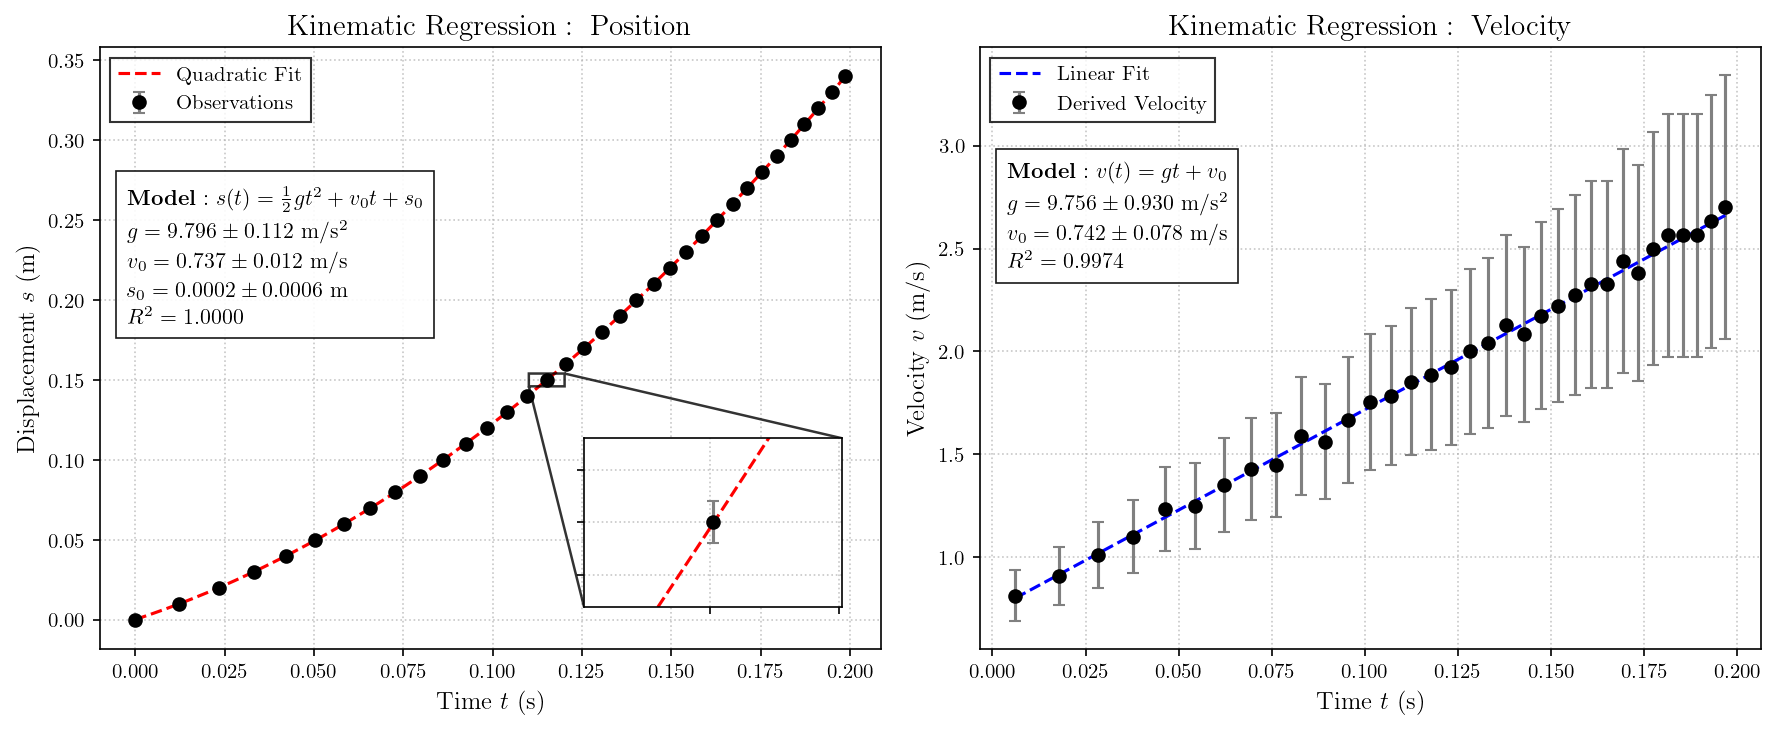
\includegraphics[width=\textwidth]{figures/fig_regression_kinematics.png}
    \caption{Trực quan hóa đồ thị hồi quy kết hợp hộp thông tin tham số.}
    \label{fig:regression_kinematics_rendering}
\end{figure}

% \begin{pitfall}{Sự phân kỳ của thuật toán tối ưu hóa}{optimization_divergence}
\begin{pitfall}{Hiện tượng phân kỳ trong thuật toán tối ưu hóa phi tuyến}{optimization_divergence}
Khi khởi chạy hàm \texttt{curve\_fit} cho các mô hình phi tuyến, thuật toán đôi khi trả về ngoại lệ \texttt{Optimal parameters not found}. Lỗi này xuất phát từ bản chất của các phương pháp tối ưu hóa lặp (ví dụ: thuật toán Levenberg-Marquardt), vốn rất nhạy cảm với miền tham số. Nếu điểm xuất phát (initial guess) mặc định (được thiết lập qua đối số \texttt{p0}) nằm quá xa so với cực tiểu toàn cục, thuật toán dễ bị kẹt tại các cực tiểu cục bộ (local minima) hoặc không hội tụ. Để giảm đáng kể rủi ro này, chương trình cần truyền vào một tập giá trị ban đầu hợp lý về mặt vật lý (ví dụ: \texttt{p0=[9.8, 0.0, 0.0]}). Giá trị $9.8$ cung cấp cho thuật toán một giá trị khởi tạo hợp lý (lực hấp dẫn), giúp thuật toán hội tụ ổn định hơn và tối ưu hóa thời gian xử lý.
\end{pitfall}